% Preamble:
% \usepackage{tikz}
% \usepackage{subcaption}

\begin{figure}[ht]
\centering

% ---------------- (a) Tree ----------------
\begin{subfigure}[t]{0.48\textwidth}
\centering
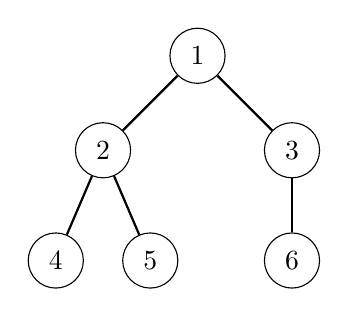
\begin{tikzpicture}[
  v/.style={circle, draw, minimum size=7mm},
  e/.style={thick}
]
\node[v] (1) at (0,0) {1};
\node[v] (2) at (-1.2,-1.2) {2};
\node[v] (3) at (1.2,-1.2) {3};
\node[v] (4) at (-1.8,-2.6) {4};
\node[v] (5) at (-0.6,-2.6) {5};
\node[v] (6) at (1.2,-2.6) {6};

\draw[e] (1)--(2);
\draw[e] (1)--(3);
\draw[e] (2)--(4);
\draw[e] (2)--(5);
\draw[e] (3)--(6);
\end{tikzpicture}
\caption{Tree}
\label{fig:tree}
\end{subfigure}
\hfill
% ---------------- (b) Forest ----------------
\begin{subfigure}[t]{0.48\textwidth}
\centering
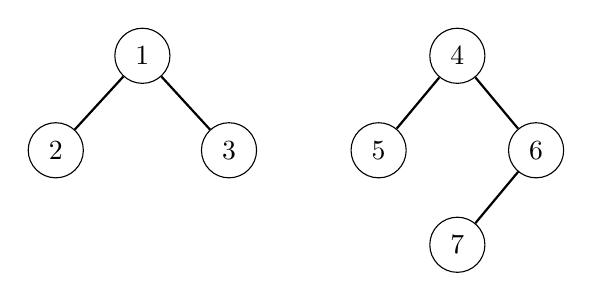
\begin{tikzpicture}[
  v/.style={circle, draw, minimum size=7mm},
  e/.style={thick}
]
% Tree 1
\node[v] (1) at (0,0) {1};
\node[v] (2) at (-1.1,-1.2) {2};
\node[v] (3) at (1.1,-1.2) {3};
\draw[e] (1)--(2);
\draw[e] (1)--(3);

% Tree 2 (disjoint)
\node[v] (4) at (4,0) {4};
\node[v] (5) at (3.0,-1.2) {5};
\node[v] (6) at (5.0,-1.2) {6};
\node[v] (7) at (4.0,-2.4) {7};
\draw[e] (4)--(5);
\draw[e] (4)--(6);
\draw[e] (6)--(7);
\end{tikzpicture}
\caption{Forest (disjoint trees)}
\label{fig:forest}
\end{subfigure}

\vspace{6mm}

% ---------------- (c) Directed tree / arborescence ----------------
\begin{subfigure}[t]{0.48\textwidth}
\centering
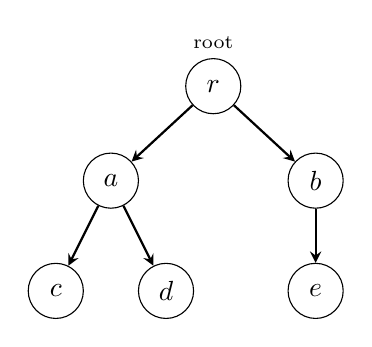
\begin{tikzpicture}[
  v/.style={circle, draw, minimum size=7mm},
  e/.style={->, thick, >=stealth}
]
\node[v] (r) at (0,0) {$r$};
\node[v] (a) at (-1.3,-1.2) {$a$};
\node[v] (b) at (1.3,-1.2) {$b$};
\node[v] (c) at (-2.0,-2.6) {$c$};
\node[v] (d) at (-0.6,-2.6) {$d$};
\node[v] (e1) at (1.3,-2.6) {$e$};

\draw[e] (r) -- (a);
\draw[e] (r) -- (b);
\draw[e] (a) -- (c);
\draw[e] (a) -- (d);
\draw[e] (b) -- (e1);

% root label
\node[draw=none, font=\scriptsize] at (0,0.55) {root};
\end{tikzpicture}
\caption{Directed tree (arborescence)}
\label{fig:arborescence}
\end{subfigure}
\hfill
% ---------------- (d) DAG ----------------
\begin{subfigure}[t]{0.48\textwidth}
\centering
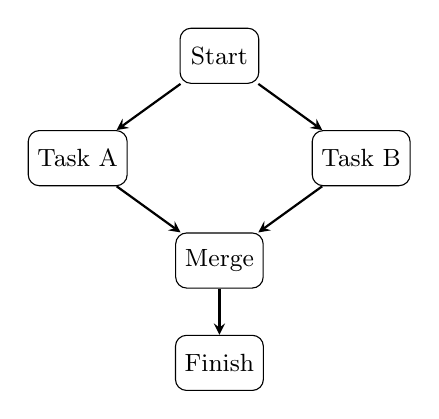
\begin{tikzpicture}[
  v/.style={rectangle, draw, rounded corners, minimum width=10mm, minimum height=7mm, font=\small},
  e/.style={->, thick, >=stealth}
]
\node[v] (s) at (0,0) {Start};
\node[v] (x) at (-1.8,-1.3) {Task A};
\node[v] (y) at (1.8,-1.3) {Task B};
\node[v] (z) at (0,-2.6) {Merge};
\node[v] (t) at (0,-3.9) {Finish};

\draw[e] (s) -- (x);
\draw[e] (s) -- (y);
\draw[e] (x) -- (z);
\draw[e] (y) -- (z);
\draw[e] (z) -- (t);
\end{tikzpicture}
\caption{DAG (no directed cycles)}
\label{fig:dag}
\end{subfigure}

\caption{Examples: (a) a tree (connected and acyclic), (b) a forest (disjoint set of trees), (c) a directed tree/arborescence (unique directed path from root to each node), and (d) a DAG (directed acyclic graph).}
\label{fig:tree-forest-arborescence-dag}
\end{figure}
